\documentclass[tikz, border=0pt]{standalone}
\usepackage{tikz}
\usepackage{amssymb}
% 必须加载 arrows.meta 库才能使用 Stealth 和 scale 参数
\usetikzlibrary{arrows.meta} 

% ==================================================================
% --- 你的核心色板 (保持不变) ---
% ==================================================================
\definecolor{WLTeal}{HTML}{00897B}   
\definecolor{WLViolet}{HTML}{5E35B1} 
\definecolor{WLBlue}{HTML}{1565C0}   
\definecolor{WLGray}{HTML}{546E7A}   
\definecolor{BG_Teal}{HTML}{E0F2F1}  
\definecolor{BG_Blue}{HTML}{E3F2FD}  

\begin{document}

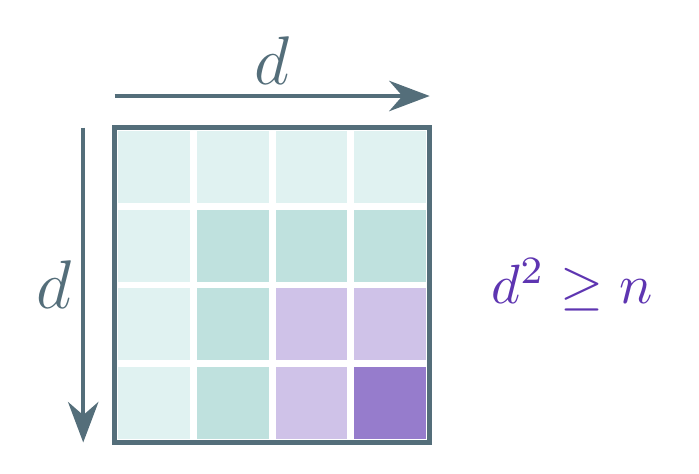
\begin{tikzpicture}[
    font=\sffamily\bfseries, 
    % 这里设置默认箭头样式,防止哪里漏写
    >=Stealth,
    % 全局线条加粗
    line width=1.5pt 
]

    \def\d{4}

    % --- 1. 色块填充 ---
    \foreach \i/\col in {
        0/BG_Teal, 
        1/WLTeal!25, 
        2/WLViolet!30, 
        3/WLViolet!65
    } {
        \fill[\col, draw=none] (\i, 0) rectangle (\d, \d-\i);
    }

    % --- 2. 网格线 ---
    \draw[step=1, white, line width=2.5pt] (0,0) grid (\d,\d);

    % --- 3. 外边框 ---
    \draw[WLGray, line width=2pt] (0,0) rectangle (\d,\d);

    % --- 4. 标注与箭头 (修复报错部分) ---
    \begin{scope}[WLGray]
        % 修复:将 [->, {Stealth...}] 改为 [-{Stealth...}]
        % 语法含义:线条(-)连接到箭头尖端({Stealth...})
        
        % 上方箭头
        \draw[-{Stealth[scale=1.5]}] (0, \d + 0.4) -- (\d, \d + 0.4);
        \node[above] at (\d/2, \d + 0.4) {\Huge $d$};
        
        % 左侧箭头
        \draw[-{Stealth[scale=1.5]}] (-0.4, \d) -- (-0.4, 0);
        \node[left] at (-0.4, \d/2) {\Huge $d$};
    \end{scope}

    % --- 5. 右侧公式 ---
    \node[right, WLViolet, scale=2.0] at (\d + 0.5, \d/2) {$d^2 \ge n$};

\end{tikzpicture}

\end{document}